\begin{frame}
    \frametitle{Radiation Modeling}
    \only<1>{
        \begin{itemize}
            \item \textbf{Irradiance:} instantaneous flux of solar radiation falling on a surface (\si{\watt\per\square\meter})
            \item \textbf{Radiation:} accumulated energy flux incident on the surface over a given period of time (\si{\watt\hour\per\square\meter})
        \end{itemize}
    }
    \only<2>{
        Solar radiation received by a surface can be divided into direct (B), diffuse (D), and reflected (R) components. The sum of these components is the  global radiation (G).
        \vspace*{0.5cm}
        \begin{figure}
            \centering
            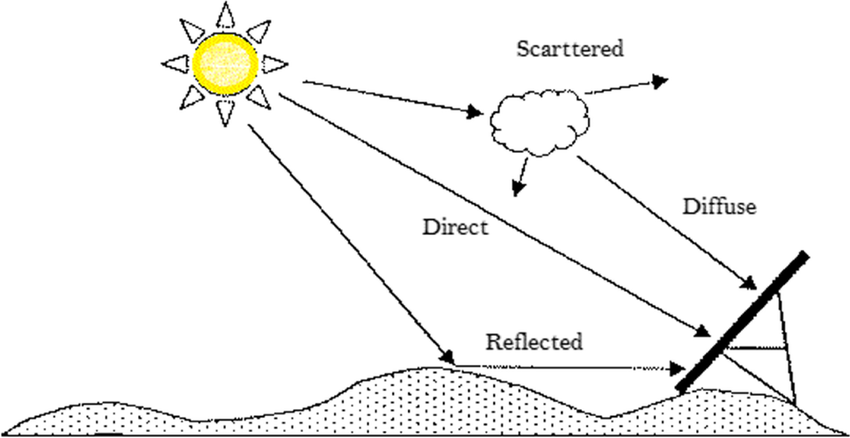
\includegraphics{Radiation_components.png}
        \end{figure}
    }
\end{frame}